\chapter{Large Language Models}
\pagestyle{fancy}\lhead{\textbf \footnotesize\it{Large Language Models}}
\pagestyle{fancy}\chead{} \pagestyle{fancy}\rhead{}
\pagestyle{fancy}\lfoot{\textbf {\small\it{Univ-Mascara/Computer Science: 2024}}} 
\pagestyle{fancy}\cfoot{} \pagestyle{fancy}\rfoot{\thepage}
%%%%%%%%%%%%%%%%%%%%%%%%%%%%%%%%%%%%%%%%
\section{Overview}\label{start4}
This chapter provides an in-depth exploration into the transformative landscape of large language models (LLMs) and their pivotal role in revolutionizing natural language processing (NLP) and machine translation (MT). 

We begin by delving into the foundational architecture of LLMs, notably Transformers, BERT, and GPT, which have reshaped the understanding of linguistic patterns and relationships. 
Within this context, we examine how LLMs, particularly BERT and GPT, have evolved to address bidirectional context understanding and generative text tasks, respectively. 

Furthermore, we explore the application of LLMs in MT, showcasing variants like BERT, T5, and ChatGPT, which demonstrate promising potential in overcoming language barriers and enhancing translation accuracy. 

Following this exploration, we present a comprehensive section on related work, offering insights into the latest research and advancements in the field of LLM-based MT.

\section{Transformers}\label{sec:transformers}
While LSTMs and GRUs alleviate the issue of losing distant information inherent in simple RNNs, they are unable to leverage parallel computing resources due to their sequential nature. 
This limitation is addressed by Transformers, as introduced by \cite{vaswani17}.
Transformers revolutionize sequence processing by completely replacing RNNs. 
They operate by mapping sequences of input vectors $(x_1, x_2, ..., x_m)$ to sequences of output vectors $(y_1, y_2, ..., y_n)$ through stacks of network layers featuring customized connections of basic feed-forward networks and self-attentions. 
Unlike RNNs, Transformers enable the extraction and utilization of information from broader contexts through self-attention mechanisms, without the need for recurrent intermediary connections.
\begin{figure}
	\centering
	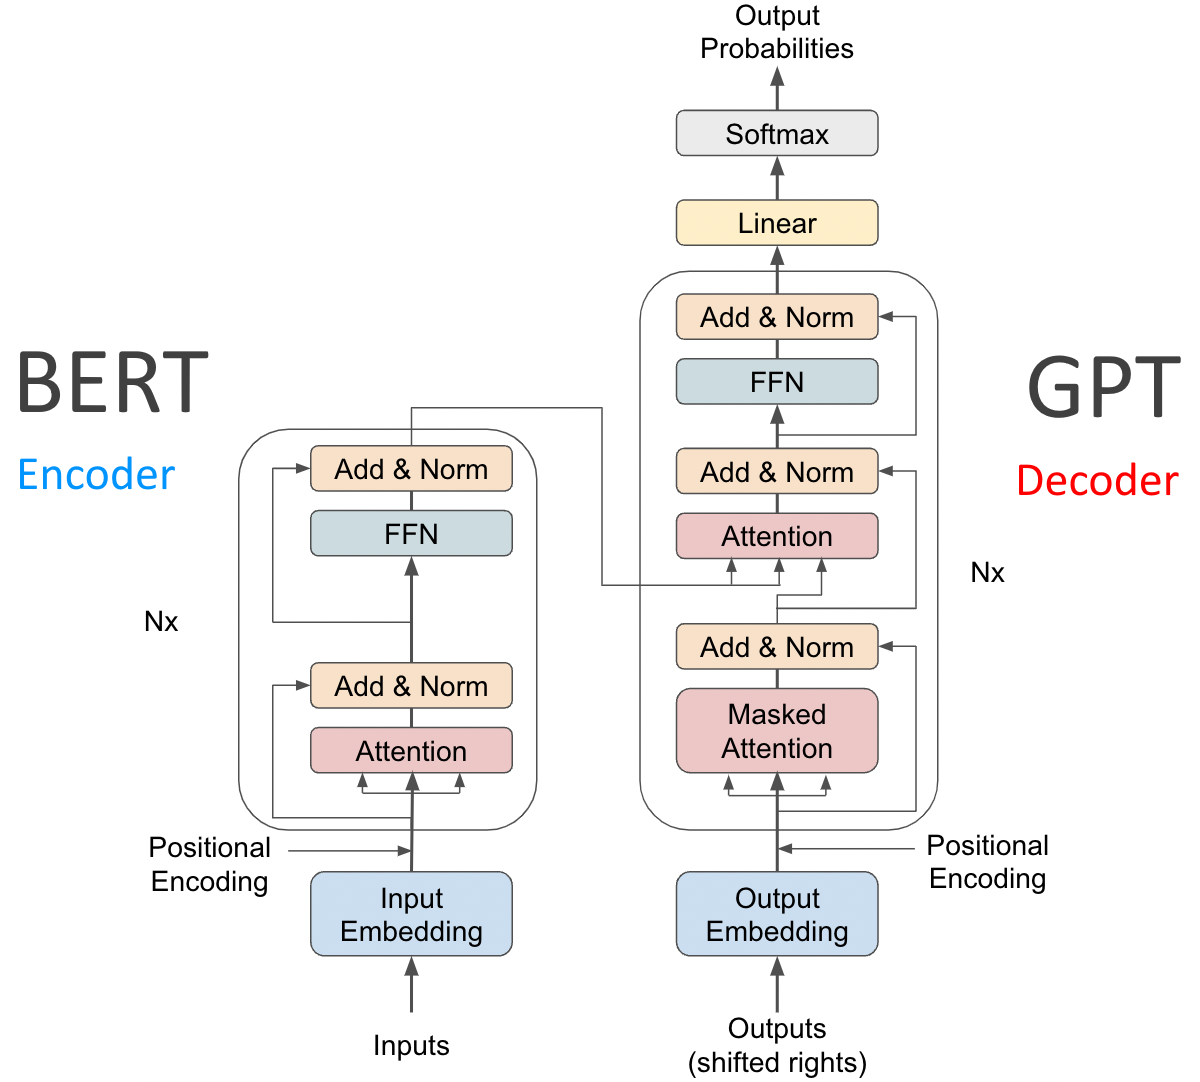
\includegraphics[width=0.5\linewidth]{Figures/Transformer}
	\caption{Transformer architecture adapted from \cite{vaswani17}}
	\label{fig:transformer}
\end{figure}

The Transformer, as depicted in Figure~\ref{fig:transformer}, is a sequence-to-sequence (Seq2Seq) network that captures sequential information through stacked self-attention and cross-attention layers. 
The output $O$ of each attention sub-layer is calculated using scaled multiplicative formulations, as defined by:
\begin{equation}
	A = (QW^Q)(KW^K)^T/\sqrt{d};\;\;\;   
	Att(Q, K, V ) = softmax(A)(V W^V )
\end{equation}
\begin{equation}
	O = Att(Q, K, V )W^O
\end{equation}
Where, $Q = (q_1, ..., q_{l_q}) \in \mathbb{R}^{l_q \times d}$,$K = (k_1, ..., k_{l_k}) \in \mathbb{R}^{l_k \times d}$, $V = (v_1, ..., v_{l_k}) \in \mathbb{R}^{l_k \times d}$ represent matrices of query, key, and value vectors respectively. Additionally, $W^Q$, $W^K$, $W^V$, and $W^O \in \mathbb{R}^{d \times d}$ denote the associated trainable weight matrices. $A$ signifies the affinity scores (or attention scores) between queries and keys, while $Att(Q, K, V)$ represents the attention vectors.
In practical applications, multi-head attention is utilized rather than single-head attention. 
Here, the hidden dimension $d$ is divided into $h$ segments, each processed independently through an attention layer before being amalgamated back together. 
Subsequently, the final output of a Transformer layer is determined as follows:
\begin{equation}
	\phi(A, Q) = LN(FFN(LN(O + Q)) + LN(O + Q))
\end{equation}
Here, $\phi$ denotes the standard sequential operations of a Transformer layer incorporating layer normalization (LN) and feed-forward (FFN) layers. The feed-forward layers essentially consist of sequences of fully connected layers interspersed with $ReLU$ activation, which are applied to each token's latent vector separately.

Since attention layers are insensitive to order, implying that the arrangement of key sequences doesn't influence the outcome of a specific query, it's crucial to introduce some form of ordering information for the model to grasp temporal characteristics of the input. 
To address this, the Transformer integrates positional encoding into the word embeddings immediately after the embedding layer and before the initial attention layer. 
This positional encoding relies on sine (Equation~\ref{eqn:E_sin}) and cosine (Equation~\ref{eqn:E_cos}) functions and is defined as follows:
\begin{equation}
	E(pos, 2i) = \sin(pos/10000^{2i/d})
	\label{eqn:E_sin}
\end{equation}
\begin{equation}
	E(pos, 2i+1) = \cos(pos/10000^{2i/d})
	\label{eqn:E_cos}
\end{equation}
Here, $pos$ denotes the position of the word within the sequence, while $i$ is the dimension.

\section{Large Language Models}
At the forefront of Natural Language Processing (NLP) stands a novel class of models termed Large Language Models (LLMs). 
These intricate artificial neural networks undergo training on massive volumes of textual data. Diverging from conventional NLP models tailored to specific tasks, LLMs acquire a broader comprehension of linguistic structures and correlations. 
This versatility enables them to undertake a diverse array of tasks, encompassing sentiment analysis, question answering, text summarization, and even creative writing. 
Notably, LLMs have significantly propelled the field of machine translation, a critical conduit between languages. 
Through extensive analysis of translated text datasets, these models can grasp the nuances inherent in different languages, yielding translations that are notably more precise and natural compared to traditional rule-based methodologies. 
However, the effectiveness of LLMs crucially depends on the caliber and extent of their training data. 
Greater diversity and comprehensiveness in the dataset enhance the model's understanding of the intricacies of human language. 
This has led to the exploration of specific LLM architectures such as BERT, mBERT, and GPT, among others, each contributing to the ongoing evolution of NLP and machine translation through their distinctive training methods and capabilities.

\subsection{BERT}
BERT, or Bidirectional Encoder Representations from Transformers, emerged as a groundbreaking pre-training method in the realm of Natural Language Processing (NLP). 
Unveiled by \cite{devlin18}, BERT reshaped the landscape by achieving top-tier performance across a diverse array of NLP tasks. 
Its standout feature lies in its adeptness at leveraging extensive, unlabeled text corpora during pre-training. 
Unlike earlier approaches that relied on task-specific labeled data, BERT follows a two-phase strategy. 
Initially, it undergoes pre-training on tasks like masked language modeling and next sentence prediction, exposing it to various linguistic structures and relationships. 
This equips the model with a robust grasp of word semantics and contextual nuances, forming a strong foundation for fine-tuning on specific tasks. 
BERT produces embeddings as its output, rather than predicting the next words in a sequence. 
To utilize these embeddings, additional layers must be added on top, such as those for text classification or question answering tasks.

BERT's architectural backbone relies on the Transformer encoder (see Figure~\ref{fig:transformer}), a potent neural network architecture introduced by \cite{vaswani17}. 
Unlike traditional sequential models, the Transformer enables parallel processing of entire input sentences, facilitating the capture of long-range dependencies essential for tasks such as sentiment analysis and question answering (see Figure~\ref{fig:bert}). 
Notably, BERT employs a pre-trained encoder model and foregoes the decoder component typically found in sequence-to-sequence models like those used in machine translation. 
This design choice underscores BERT's focus on comprehending text rather than generating new sequences. A key contributor to BERT's efficacy is the scale of its pre-training data, drawn from vast text corpora like BookCorpus and English Wikipedia. 
\begin{figure}
	\centering
	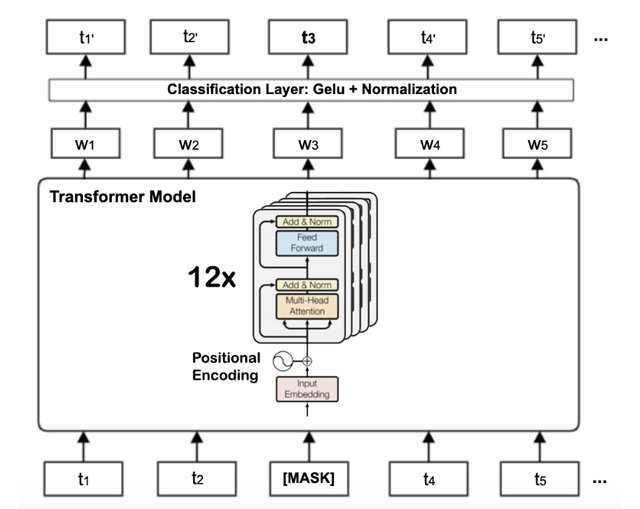
\includegraphics[width=0.7\linewidth]{Figures/BERT}
	\caption{BERT base architecture with twelve encoder blocks, adapted from \cite{khalid21}.}
	\label{fig:bert}
\end{figure}

While BERT's original training was centered on English, subsequent research has explored its applicability to multilingual NLP tasks. 
mBERT, short for multilingual BERT, extends the capabilities of BERT to encompass tasks spanning multiple languages. It inherits BERT's architecture but undergoes training on an extensive dataset containing text samples from a staggering 104 languages.
Efforts such as mBERT have demonstrated the feasibility of fine-tuning pre-trained models across multiple languages, showcasing BERT's potential for cross-lingual NLP endeavors\cite{pires19}.

\subsection{GPT}
In contrast to BERT's emphasis on pre-training encoders, Generative Pre-trained Transformer (GPT) models offer a compelling alternative for tasks involving text generation. 
Introduced by OpenAI\footnote{https://openai.com/}, GPT utilizes a decoder-based architecture derived from the Transformer family. 
This design enables GPT to excel in generating various forms of creative text, including poems, code, scripts, musical compositions, and even realistic chat dialogues \cite{radford18}.

Unlike BERT, GPT is predominantly trained on a single, extensive dataset consisting of text and code. 
The initial GPT model, GPT-1, was trained on a dataset compiled from internet sources, while subsequent versions like GPT-2 and GPT-3 have utilized progressively larger and more diverse datasets. 
Focusing on a single language, typically English, allows GPT to grasp statistical patterns and sequential dependencies within the text, thereby generating text of human-like quality that can often be mistaken for content written by humans.

The fundamental architecture of GPT relies on a Transformer decoder (see Figure~\ref{fig:transformer}). 
Unlike encoders that process the entire input sequence simultaneously, decoders handle the input sequence one element (word) at a time. 
This iterative approach enables GPT to predict the next word in a sequence based on previously generated words and the overall context, making it proficient in tasks like text summarization, machine translation, and creative writing, where generating coherent text is crucial.
\begin{figure}
	\centering
	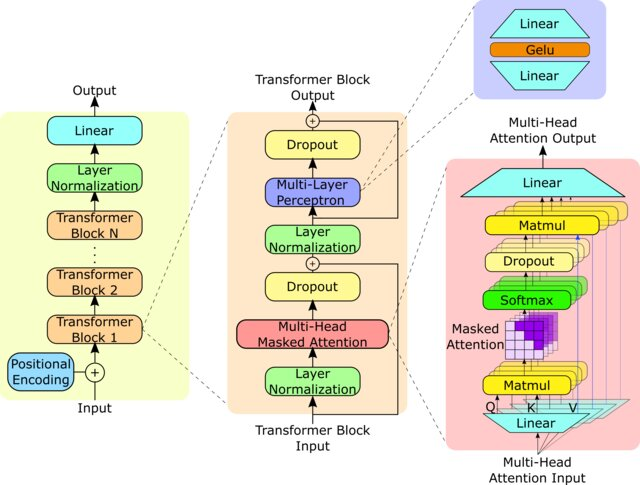
\includegraphics[width=0.7\linewidth]{Figures/GPT2}
	\caption[]{GPT-2 model architecture adapted from \cite{yang23}. }
	\label{fig:gpt2}
\end{figure}

In language scenarios, decoders play a crucial role in generating subsequent words, such as in text translation or story generation, where the outputs are words with probabilities.
Decoders integrate attention mechanisms, employing them twice in their operation. Initially, during model training, they utilize Masked Multi-Head Attention, where only the initial words of the target sentence are revealed to prevent the model from cheating during learning. This approach resembles the MASK concept introduced in BERT.
Subsequently, decoders employ Multi-Head Attention \cite{liu21}, similar to how it is utilized in the encoder. Transformer-based models incorporating both encoders and decoders employ a technique for enhanced efficiency. The output of the encoders serves as input to the decoders, specifically as keys and values. Decoders can then make queries to locate the most relevant keys. This facilitates tasks such as comprehending the original sentence's meaning and translating it into other languages, even when the resulting word count and order vary.
Figure~\ref{fig:gpt2} illustrates the structure of GPT-2, consisting of N Transformer decoder blocks. Each block is equipped with multi-head masked attention, multi-layer perceptrons, normalization, and dropout layers. Residual connections link these blocks, enhancing the model's ability to learn from earlier inputs. The multi-head masked attention mechanism employs Q, K, and V vectors for calculating attention scores, effectively capturing and encoding the sequential relationships within the data.
%While GPT models are primarily trained on a single language, ongoing research is exploring their adaptability to multilingual tasks. 
%Techniques such as multilingual fine-tuning allow GPT models to be adjusted for generating text in multiple languages. 
%However, due to their single-language focus during pre-training, GPT models generally exhibit lower performance on multilingual tasks compared to models like mBERT, which are explicitly designed for handling multiple languages.

\section{LLM-based Machine Translation}
Unlike conventional rule-based methodologies that depend on predetermined linguistic principles, Large Language Models (LLMs) utilize extensive real-world translation datasets to grasp the intricacies and statistical regularities of language \cite{brants07}. This enables them to generate translations that are more natural-sounding and precise compared to traditional techniques.

A significant advantage of LLM-based MT lies in its capacity to comprehend context. By analyzing extensive sets of translated texts, LLMs can discern the connections between words, phrases, and the overall context of a sentence. This contextual comprehension empowers them to produce translations that not only adhere to grammatical rules but also capture the intended meaning and nuances of the source language.

Numerous research studies have investigated the efficacy of LLMs in MT. For example, the study conducted by  showcases how LLMs can achieve superior performance on diverse language pairs, sometimes outperforming traditional statistical MT approaches.

Nevertheless, LLM-based MT encounters certain challenges. One concern is the potential presence of bias in the training data, which may manifest in the translated output \cite{wang24}. 
Translating content into English may enhance multilingual NLP tasks for English-centric LLMs, yet it's not always the best approach, particularly for tasks requiring deep cultural and linguistic comprehension. 
Using the native language directly often yields better results by capturing cultural nuances more effectively \cite{liu24}.
Additionally, LLMs can pose computational challenges due to their extensive size and complexity, making training and deployment resource-intensive \cite{yang24}.
Despite these hurdles, LLM-based MT offers a promising avenue for seamless cross-lingual communication. As research advances and training datasets expand, we anticipate further progress in this dynamic field.

\subsection{BART}
BART (Bidirectional and Autoregressive Transformer) arises as a potent Large Language Model, differentiating itself from GPT's focus on decoders and BERT's emphasis on encoders. 
It achieves this by integrating both encoder and decoder elements, enabling it to tackle tasks related to both Natural Language Generation (NLG) and Natural Language Understanding (NLU). 
This dual structure synergizes the comprehensive understanding capabilities of the encoder with the fluent generative abilities of the decoder. 

As highlighted in \cite{lewis19}, BART's architecture enables it to deliver superior performance in MT by thoroughly grasping the source language context with its encoder and producing coherent translations with its decoder. 
The ability to pre-train on extensive multilingual datasets further enhances BART's proficiency in handling a wide array of language pairs, positioning it as an effective solution for overcoming language barriers.
Figure~\ref{fig:bart} illustrates the BART model adapted for MT. In this scenario, a supplementary encoder is introduced to substitute word embeddings within BART. This new encoder has the flexibility to utilize a separate vocabulary.
\begin{figure}[h]
	\centering
	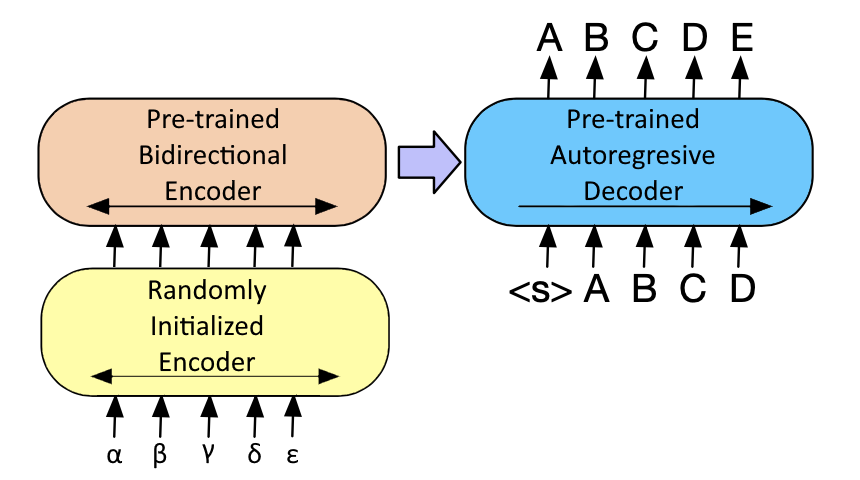
\includegraphics[width=0.7\linewidth]{Figures/Bart}
	\caption{Fine tuning BART for machine translation.}
	\label{fig:bart}
\end{figure}

\subsection{T5}
T5, or Text-to-Text Transfer Transformer, emerges as a formidable player in the landscape of LLM-based MT. 
Unlike models such as BERT, which concentrate on pre-training encoders, or GPT, which prioritize decoders, T5 takes a unified approach. 
It employs a single Transformer-based architecture that can be fine-tuned for various NLP tasks, including machine translation (see Figure~\ref{fig:t5}).

%This design, outlined in the paper "Exploring the Limits of Language Learning with a Unified Text-to-Text Transformer" by Raffel et al. (2020), grants T5 exceptional adaptability in addressing MT challenges. 
The model can be trained on extensive multilingual text and code datasets, enabling it to comprehend the nuances of different languages and perform effective translations between them. 
Moreover, T5's capability to adjust to diverse NLP tasks equips it to handle a wide range of translation scenarios, from straightforward sentence translations to intricate document summarization with translation components. 
This versatility positions T5 as a valuable resource for applications necessitating seamless and nuanced language transfer across various domains.
\begin{figure}
	\centering
	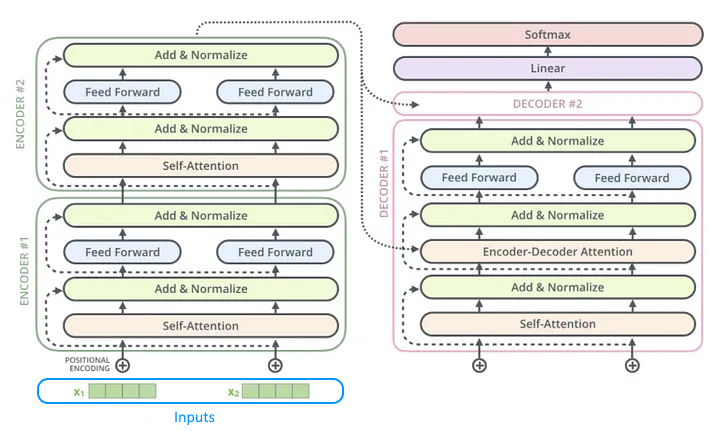
\includegraphics[width=0.7\linewidth]{Figures/T5}
	\caption{T5 model architecture adapted from \cite{wang23}.}
	\label{fig:t5}
\end{figure}

\subsection{ChatGPT}
While ChatGPT demonstrates remarkable proficiency in generating diverse text formats creatively, its utility in MT is circumscribed by certain constraints \cite{lyu23}. 
Unlike specialized models like BART or T5 tailored explicitly for managing both source and target languages, ChatGPT's fundamental capability resides in its decoder-centric architecture. 
This design excels in text generation based on provided prompts or contexts, rendering it suitable for tasks such as creative writing or text summarization.
owever, for achieving precise and natural-sounding translations, comprehending the context of the source language is imperative. 
ChatGPT's primary emphasis on text generation within a single language, typically English (GPT data proportion is only 7\% non-English \cite{pourkamali24}), constrains its capacity to fully comprehend the subtleties and intricacies involved in translating between diverse languages. 
Therefore, while it can generate text in various languages based on the input it receives, its proficiency in languages other than English may vary depending on factors such as the availability and diversity of training data in those languages.

While some research endeavors explore the potential of adapting ChatGPT for multilingual purposes \cite{brown20, lu23, peng23, pourkamali24}, it has been observed that ChatGPT often generates inaccurate outputs and hallucinates for non-English-centric machine translation tasks \cite{peng23}. 
Its performance generally lags behind models like mBERT or BART, specifically designed for multilingual understanding and translation. 
Additionally, studies have shown that while ChatGPT can compete with commercial translation products such as Google Translate and Microsoft Translator for high-resource languages, it exhibits limited capabilities for low-resource and distant languages \cite{peng23, hendy23, jiao23, pourkamali24}.
\begin{figure}
	\centering
	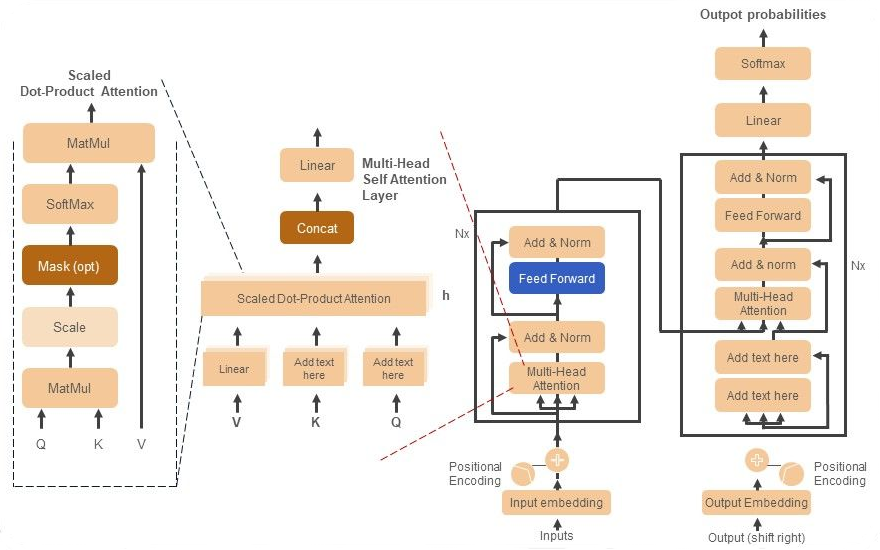
\includegraphics[width=1.0\linewidth]{Figures/ChatGPT-model}
	\caption{Transformer architecture of ChatGPT}
	\label{fig:chatgpt-model}
\end{figure}

\section{Related Work}
\hl{.....................................................................}

\cite{brown20}
\cite{lu23}
\cite{peng23}
\cite{hendy23}
\cite{jiao23}
\cite{pourkamali24}
\cite{jiang24}
\\
\hl{.....................................................................}

\section{Summary}
In this chapter, we delved into the transformative impact of large language models (LLMs), notably focusing on the advancements brought forth by models such as Transformers, BERT, and GPT within the realm of natural language processing (NLP). 
These models, built upon Transformer architectures, have revolutionized NLP tasks by learning intricate linguistic patterns and relationships. 
Particularly, BERT and GPT represent pioneering models, with BERT excelling in understanding bidirectional context and GPT specializing in generative tasks. 

Leveraging LLMs for machine translation (MT), variants like BERT, T5, and ChatGPT demonstrate promising capabilities in bridging language barriers and enhancing translation accuracy. 
However, challenges persist, including the need for diverse and extensive training data and mitigating biases inherent in these models. 
Nevertheless, ongoing research endeavors continue to explore advancements and refine techniques in leveraging LLMs for MT, underscoring the dynamic evolution of NLP and MT technologies. 